\subsection{Hall Sensor}
There are two hall sensors implemented on the vehicle, one by each drive gear. Four magnets are placed on each drive gear, with a quarter turn between each. The hall sensor is illustrated in \figref{HallSensor}.

\begin{figure}[H]
	\centering
	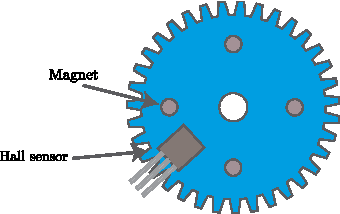
\includegraphics[scale=1.2]{figures/hallSensorDrawing.pdf}
	\caption{Illustration of the drive gear, with the magnets and the hall sensor. The hall sensor is placed stationary beside the rotating gear\cite{KHSoerensen}.}
	\label{HallSensor}
\end{figure}
%
A hall sensor is affected by magnetic fields. When the field is significantly larger than the ambient fields a pulse is generated. This gives a voltage output each time one of the magnets is in front of the hall sensor. Therefore each time the drive gear makes a quarter of a turn a voltage signal is generated.

%As the distance between each magnet is not exactly a quarter of a turn, the calculations of the pulses received from the Hall sensor, is processed for each magnet independently.
%By measuring the time between five outputs, as the first and the fifth output is from the same magnet, the time of a whole rotation of the gear can be found. By knowing the distance the vehicle travels for a full rotation of the gear, the speed can be calculated.
%
%When the vehicle is starting to move, the speed of the first turn of the gear can not be calculated. This is because two signal from the same magnet are needed before the speed can be calculated. So the first four output from the hall sensor will be saved and at the fifth output, after a whole turn, the speed related to the first magnet will be calculated.\\
%
%The hall sensors are used to measure the speed of the two belts, which will run at different speeds when the vehicle is turning. Now that the components linked to the velocity  are described, the steering material will be analysed.
